\documentclass[]{book}
\usepackage{lmodern}
\usepackage{amssymb,amsmath}
\usepackage{ifxetex,ifluatex}
\usepackage{fixltx2e} % provides \textsubscript
\ifnum 0\ifxetex 1\fi\ifluatex 1\fi=0 % if pdftex
  \usepackage[T1]{fontenc}
  \usepackage[utf8]{inputenc}
\else % if luatex or xelatex
  \ifxetex
    \usepackage{mathspec}
  \else
    \usepackage{fontspec}
  \fi
  \defaultfontfeatures{Ligatures=TeX,Scale=MatchLowercase}
\fi
% use upquote if available, for straight quotes in verbatim environments
\IfFileExists{upquote.sty}{\usepackage{upquote}}{}
% use microtype if available
\IfFileExists{microtype.sty}{%
\usepackage{microtype}
\UseMicrotypeSet[protrusion]{basicmath} % disable protrusion for tt fonts
}{}
\usepackage[margin=1in]{geometry}
\usepackage{hyperref}
\hypersetup{unicode=true,
            pdftitle={Legal Education Analysis in R},
            pdfauthor={Richard G. Gardiner},
            pdfborder={0 0 0},
            breaklinks=true}
\urlstyle{same}  % don't use monospace font for urls
\usepackage{natbib}
\bibliographystyle{apalike}
\usepackage{color}
\usepackage{fancyvrb}
\newcommand{\VerbBar}{|}
\newcommand{\VERB}{\Verb[commandchars=\\\{\}]}
\DefineVerbatimEnvironment{Highlighting}{Verbatim}{commandchars=\\\{\}}
% Add ',fontsize=\small' for more characters per line
\usepackage{framed}
\definecolor{shadecolor}{RGB}{248,248,248}
\newenvironment{Shaded}{\begin{snugshade}}{\end{snugshade}}
\newcommand{\KeywordTok}[1]{\textcolor[rgb]{0.13,0.29,0.53}{\textbf{#1}}}
\newcommand{\DataTypeTok}[1]{\textcolor[rgb]{0.13,0.29,0.53}{#1}}
\newcommand{\DecValTok}[1]{\textcolor[rgb]{0.00,0.00,0.81}{#1}}
\newcommand{\BaseNTok}[1]{\textcolor[rgb]{0.00,0.00,0.81}{#1}}
\newcommand{\FloatTok}[1]{\textcolor[rgb]{0.00,0.00,0.81}{#1}}
\newcommand{\ConstantTok}[1]{\textcolor[rgb]{0.00,0.00,0.00}{#1}}
\newcommand{\CharTok}[1]{\textcolor[rgb]{0.31,0.60,0.02}{#1}}
\newcommand{\SpecialCharTok}[1]{\textcolor[rgb]{0.00,0.00,0.00}{#1}}
\newcommand{\StringTok}[1]{\textcolor[rgb]{0.31,0.60,0.02}{#1}}
\newcommand{\VerbatimStringTok}[1]{\textcolor[rgb]{0.31,0.60,0.02}{#1}}
\newcommand{\SpecialStringTok}[1]{\textcolor[rgb]{0.31,0.60,0.02}{#1}}
\newcommand{\ImportTok}[1]{#1}
\newcommand{\CommentTok}[1]{\textcolor[rgb]{0.56,0.35,0.01}{\textit{#1}}}
\newcommand{\DocumentationTok}[1]{\textcolor[rgb]{0.56,0.35,0.01}{\textbf{\textit{#1}}}}
\newcommand{\AnnotationTok}[1]{\textcolor[rgb]{0.56,0.35,0.01}{\textbf{\textit{#1}}}}
\newcommand{\CommentVarTok}[1]{\textcolor[rgb]{0.56,0.35,0.01}{\textbf{\textit{#1}}}}
\newcommand{\OtherTok}[1]{\textcolor[rgb]{0.56,0.35,0.01}{#1}}
\newcommand{\FunctionTok}[1]{\textcolor[rgb]{0.00,0.00,0.00}{#1}}
\newcommand{\VariableTok}[1]{\textcolor[rgb]{0.00,0.00,0.00}{#1}}
\newcommand{\ControlFlowTok}[1]{\textcolor[rgb]{0.13,0.29,0.53}{\textbf{#1}}}
\newcommand{\OperatorTok}[1]{\textcolor[rgb]{0.81,0.36,0.00}{\textbf{#1}}}
\newcommand{\BuiltInTok}[1]{#1}
\newcommand{\ExtensionTok}[1]{#1}
\newcommand{\PreprocessorTok}[1]{\textcolor[rgb]{0.56,0.35,0.01}{\textit{#1}}}
\newcommand{\AttributeTok}[1]{\textcolor[rgb]{0.77,0.63,0.00}{#1}}
\newcommand{\RegionMarkerTok}[1]{#1}
\newcommand{\InformationTok}[1]{\textcolor[rgb]{0.56,0.35,0.01}{\textbf{\textit{#1}}}}
\newcommand{\WarningTok}[1]{\textcolor[rgb]{0.56,0.35,0.01}{\textbf{\textit{#1}}}}
\newcommand{\AlertTok}[1]{\textcolor[rgb]{0.94,0.16,0.16}{#1}}
\newcommand{\ErrorTok}[1]{\textcolor[rgb]{0.64,0.00,0.00}{\textbf{#1}}}
\newcommand{\NormalTok}[1]{#1}
\usepackage{longtable,booktabs}
\usepackage{graphicx,grffile}
\makeatletter
\def\maxwidth{\ifdim\Gin@nat@width>\linewidth\linewidth\else\Gin@nat@width\fi}
\def\maxheight{\ifdim\Gin@nat@height>\textheight\textheight\else\Gin@nat@height\fi}
\makeatother
% Scale images if necessary, so that they will not overflow the page
% margins by default, and it is still possible to overwrite the defaults
% using explicit options in \includegraphics[width, height, ...]{}
\setkeys{Gin}{width=\maxwidth,height=\maxheight,keepaspectratio}
\IfFileExists{parskip.sty}{%
\usepackage{parskip}
}{% else
\setlength{\parindent}{0pt}
\setlength{\parskip}{6pt plus 2pt minus 1pt}
}
\setlength{\emergencystretch}{3em}  % prevent overfull lines
\providecommand{\tightlist}{%
  \setlength{\itemsep}{0pt}\setlength{\parskip}{0pt}}
\setcounter{secnumdepth}{5}
% Redefines (sub)paragraphs to behave more like sections
\ifx\paragraph\undefined\else
\let\oldparagraph\paragraph
\renewcommand{\paragraph}[1]{\oldparagraph{#1}\mbox{}}
\fi
\ifx\subparagraph\undefined\else
\let\oldsubparagraph\subparagraph
\renewcommand{\subparagraph}[1]{\oldsubparagraph{#1}\mbox{}}
\fi

%%% Use protect on footnotes to avoid problems with footnotes in titles
\let\rmarkdownfootnote\footnote%
\def\footnote{\protect\rmarkdownfootnote}

%%% Change title format to be more compact
\usepackage{titling}

% Create subtitle command for use in maketitle
\newcommand{\subtitle}[1]{
  \posttitle{
    \begin{center}\large#1\end{center}
    }
}

\setlength{\droptitle}{-2em}

  \title{Legal Education Analysis in R}
    \pretitle{\vspace{\droptitle}\centering\huge}
  \posttitle{\par}
    \author{Richard G. Gardiner}
    \preauthor{\centering\large\emph}
  \postauthor{\par}
      \predate{\centering\large\emph}
  \postdate{\par}
    \date{2019-04-11}

\usepackage{booktabs}

\begin{document}
\maketitle

{
\setcounter{tocdepth}{1}
\tableofcontents
}
\chapter{About the Book}\label{about-the-book}

The book was developed as a personal project by the author in an attempt
to store important information about different models for legal
education. Where possible, I attempt to use real law school data to show
the examples. This book is free to use within AccessLex, but I only ask
that you give attribution.

\chapter{Introduction}\label{intro}

You can label chapter and section titles using \texttt{\{\#label\}}
after them, e.g., we can reference Chapter \ref{intro}. If you do not
manually label them, there will be automatic labels anyway, e.g.,
Chapter \ref{methods}.

Figures and tables with captions will be placed in \texttt{figure} and
\texttt{table} environments, respectively.

\begin{Shaded}
\begin{Highlighting}[]
\KeywordTok{par}\NormalTok{(}\DataTypeTok{mar =} \KeywordTok{c}\NormalTok{(}\DecValTok{4}\NormalTok{, }\DecValTok{4}\NormalTok{, .}\DecValTok{1}\NormalTok{, .}\DecValTok{1}\NormalTok{))}
\KeywordTok{plot}\NormalTok{(pressure, }\DataTypeTok{type =} \StringTok{'b'}\NormalTok{, }\DataTypeTok{pch =} \DecValTok{19}\NormalTok{)}
\end{Highlighting}
\end{Shaded}

\begin{figure}

{\centering 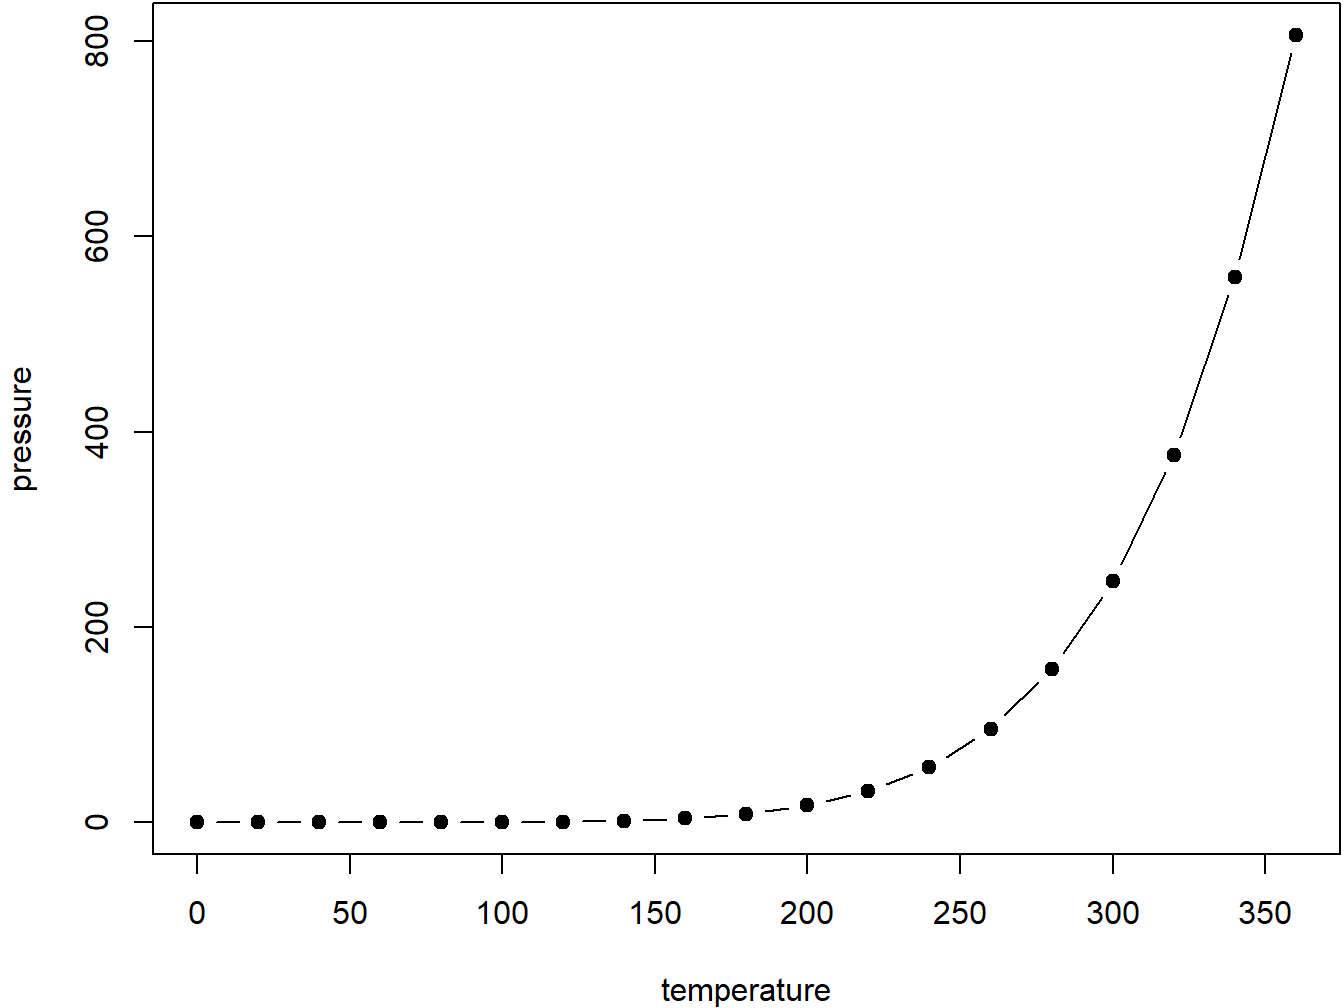
\includegraphics[width=0.8\linewidth]{Bookdown_files/figure-latex/nice-fig-1} 

}

\caption{Here is a nice figure!}\label{fig:nice-fig}
\end{figure}

Reference a figure by its code chunk label with the \texttt{fig:}
prefix, e.g., see Figure \ref{fig:nice-fig}. Similarly, you can
reference tables generated from \texttt{knitr::kable()}, e.g., see Table
\ref{tab:nice-tab}.

\begin{Shaded}
\begin{Highlighting}[]
\NormalTok{knitr}\OperatorTok{::}\KeywordTok{kable}\NormalTok{(}
  \KeywordTok{head}\NormalTok{(iris, }\DecValTok{20}\NormalTok{), }\DataTypeTok{caption =} \StringTok{'Here is a nice table!'}\NormalTok{,}
  \DataTypeTok{booktabs =} \OtherTok{TRUE}
\NormalTok{)}
\end{Highlighting}
\end{Shaded}

\begin{table}[t]

\caption{\label{tab:nice-tab}Here is a nice table!}
\centering
\begin{tabular}{rrrrl}
\toprule
Sepal.Length & Sepal.Width & Petal.Length & Petal.Width & Species\\
\midrule
5.1 & 3.5 & 1.4 & 0.2 & setosa\\
4.9 & 3.0 & 1.4 & 0.2 & setosa\\
4.7 & 3.2 & 1.3 & 0.2 & setosa\\
4.6 & 3.1 & 1.5 & 0.2 & setosa\\
5.0 & 3.6 & 1.4 & 0.2 & setosa\\
\addlinespace
5.4 & 3.9 & 1.7 & 0.4 & setosa\\
4.6 & 3.4 & 1.4 & 0.3 & setosa\\
5.0 & 3.4 & 1.5 & 0.2 & setosa\\
4.4 & 2.9 & 1.4 & 0.2 & setosa\\
4.9 & 3.1 & 1.5 & 0.1 & setosa\\
\addlinespace
5.4 & 3.7 & 1.5 & 0.2 & setosa\\
4.8 & 3.4 & 1.6 & 0.2 & setosa\\
4.8 & 3.0 & 1.4 & 0.1 & setosa\\
4.3 & 3.0 & 1.1 & 0.1 & setosa\\
5.8 & 4.0 & 1.2 & 0.2 & setosa\\
\addlinespace
5.7 & 4.4 & 1.5 & 0.4 & setosa\\
5.4 & 3.9 & 1.3 & 0.4 & setosa\\
5.1 & 3.5 & 1.4 & 0.3 & setosa\\
5.7 & 3.8 & 1.7 & 0.3 & setosa\\
5.1 & 3.8 & 1.5 & 0.3 & setosa\\
\bottomrule
\end{tabular}
\end{table}

You can write citations, too. For example, we are using the
\textbf{bookdown} package \citep{R-bookdown} in this sample book, which
was built on top of R Markdown and \textbf{knitr} \citep{xie2015}.

\chapter{Literature}\label{literature}

Here is a review of existing methods.

\section{Introducing Logit Models}\label{introducing-logit-models}

There are a number of different models that can be run with a binary
regression model (BRM) including: Linear Probability Model, Logit Model,
Probit Mode, and the Log-Log model. Most commonly we choose between the
Logit and Probit model. The logit model in the past has been the default
because the error distribution assumptions decreased the computing cost
for the probability distribution function. The decision between the
logit and probit are essentially arbitrary because the major difference
between them (the distribution of the error term) is something we cannot
tested.

When specifying a BRM, we make three main assumptions:

\begin{enumerate}
\def\labelenumi{\arabic{enumi}.}
\tightlist
\item
  The threshold for 0 is \(\tau = 0\)
\item
  The Conditional mean of \(\epsilon\) is 0: \(E(\epsilon | X) = 0\)
\item
  The conditional variance of \(\epsilon\) is constant:
  \(Var(\epsilon|X = 1)\) for probit models and
  \(Var(\epsilon|X = \pi/3)\) for logit models.
\end{enumerate}

We also assume that there is an unobserved latent variable that we
cannot fully observe, but only observe the cut point (pass/fail). We
assume that our observed x's are linearly related to the latent variable
\(y^*\).

\section{Example of Logit Model}\label{example-of-logit-model}

To show an example of a logit model at work, we will examine the titanic
dataset. Specifically we will use the titanic package and load the
titanic\_train dataset. The Dependent Variable is \texttt{Survived}
which indicates whether the person survived. Our regressors in this
analysis are: Passenger Class (\texttt{Pclass}), Sex (\texttt{Sex}), and
Age (\texttt{Age}).

\begin{Shaded}
\begin{Highlighting}[]
\KeywordTok{library}\NormalTok{(titanic)}
\KeywordTok{library}\NormalTok{(tidyverse)}
\KeywordTok{library}\NormalTok{(modelr)}

\NormalTok{titanic <-}\StringTok{ }\NormalTok{titanic_train}
\end{Highlighting}
\end{Shaded}

Our model in this case is:

\(Pr(Surv = 1) = F(\beta_0 + \beta_1Class + \beta_2Sex + \beta_3AGe + \beta_4Cabin)\)

Now lets specify the model in R:

\begin{Shaded}
\begin{Highlighting}[]
\NormalTok{model <-}\StringTok{ }\KeywordTok{glm}\NormalTok{(Survived }\OperatorTok{~}\StringTok{ }\NormalTok{Pclass }\OperatorTok{+}\StringTok{ }\NormalTok{Sex }\OperatorTok{+}\StringTok{ }\NormalTok{Age, }\DataTypeTok{family =} \StringTok{"binomial"}\NormalTok{, }\DataTypeTok{data =}\NormalTok{ titanic)}
\end{Highlighting}
\end{Shaded}

The code to run the model is very similar to that of an OLS regression.
The left hand side of the assignment operator, \texttt{\textless{}-}, is
the name of the object you are creating. On the right is the actual
model you are running. First is the \texttt{glm} which standards for
Generalized Linear Models. Just like with OLS regression, the dependent
variable is on the left of the tilde \texttt{\textasciitilde{}}. The
right side includes the independent variables. In our case the dependent
variable is Survived and the independent variables include: Pclass, Sex,
and age. The family option tells the \texttt{glm()} function the type of
dependent variable you have. In this case we have a binomial dependent
variable. Unless you specify otherwise, the default link function is the
a logit model. See this quick
\href{https://www.statmethods.net/advstats/glm.html}{page} describing
the basics of the \texttt{glm()} function. Lastly, we always have to
call our dataset.

Now let's take a look at the model.

\begin{Shaded}
\begin{Highlighting}[]
\KeywordTok{summary}\NormalTok{(model)}
\end{Highlighting}
\end{Shaded}

\begin{verbatim}
## 
## Call:
## glm(formula = Survived ~ Pclass + Sex + Age, family = "binomial", 
##     data = titanic)
## 
## Deviance Residuals: 
##     Min       1Q   Median       3Q      Max  
## -2.7270  -0.6799  -0.3947   0.6483   2.4668  
## 
## Coefficients:
##              Estimate Std. Error z value Pr(>|z|)    
## (Intercept)  5.056006   0.502128  10.069  < 2e-16 ***
## Pclass      -1.288545   0.139259  -9.253  < 2e-16 ***
## Sexmale     -2.522131   0.207283 -12.168  < 2e-16 ***
## Age         -0.036929   0.007628  -4.841 1.29e-06 ***
## ---
## Signif. codes:  0 '***' 0.001 '**' 0.01 '*' 0.05 '.' 0.1 ' ' 1
## 
## (Dispersion parameter for binomial family taken to be 1)
## 
##     Null deviance: 964.52  on 713  degrees of freedom
## Residual deviance: 647.29  on 710  degrees of freedom
##   (177 observations deleted due to missingness)
## AIC: 655.29
## 
## Number of Fisher Scoring iterations: 5
\end{verbatim}

When it comes to variables, we are looking for directionality and
significance (we are given log odds for the coefficient estimate).
Remember that the dependent variable is whether the passenger survived.
Each of our variables are negative meaning that as they increase, the
probability of surviving the titanic crash is lowered. Specifically, as
you go up in passenger class and age you are less likely to survive. Men
(compared to women) are less likely to survive. All three independent
variables are significant at virtually all accepted levels. Lastly, we
notice that our AIC is listed at 655.29. This is not informative by
itself, but can help when comparing this to other models. In its raw
form, coefficient estimates cannot tell us magnitude. Additional steps
are necessary to get predictions.

If we did, however, want to get something of substance to report in the
talbe, you can take the exponent of the estimate. This will give you the
\emph{odds ratio}. Monogan states that: ``the \emph{odds} of an event is
the ratio fo the probability the event occurs to the probabiliity it
does not occur \(\dfrac{p}{1- p}\). The odds ratio tells us the
multiplicatvie factor by which the odds will change for a unit increase
in the predictor.'' We can compute it as follows:

\begin{Shaded}
\begin{Highlighting}[]
\KeywordTok{exp}\NormalTok{(model}\OperatorTok{$}\NormalTok{coefficients[}\OperatorTok{-}\DecValTok{1}\NormalTok{])}
\end{Highlighting}
\end{Shaded}

\begin{verbatim}
##     Pclass    Sexmale        Age 
## 0.27567157 0.08028834 0.96374454
\end{verbatim}

In the code above, I excluded the intercept with \texttt{{[}-1{]}}. The
0.963 indicates that as you go up in age by 1 year, theodds that you
will survive decrease by 0.96, all else equal. If you prefer
percentages:

\begin{Shaded}
\begin{Highlighting}[]
\DecValTok{100} \OperatorTok{*}\StringTok{ }\NormalTok{(}\KeywordTok{exp}\NormalTok{(model}\OperatorTok{$}\NormalTok{coefficients[}\OperatorTok{-}\DecValTok{1}\NormalTok{])}\OperatorTok{-}\DecValTok{1}\NormalTok{)}
\end{Highlighting}
\end{Shaded}

\begin{verbatim}
##     Pclass    Sexmale        Age 
## -72.432843 -91.971166  -3.625546
\end{verbatim}

In this case as you increase in age, your odds of surviving decrease by
3.6\%.

\section{Adding Predictions}\label{adding-predictions}

Given that the direct output of a logit model is not particularly
helpful. It is nice to create graphs of predicted probabilities. These
graphs, generally, create a simulated dataset that is similar to the
dataset used to create the model, but will vary one variable while
holding the others constant.

The cleanest way that I know of how to make a new dataset is to use the
\texttt{data\_grid}. The code below calls our original dataset
\texttt{titanic}, then calls the \texttt{data\_grid} function. Within
the data\_grid function you call the variable you wish to vary, in our
case I picked \texttt{Age}. the \texttt{.model\ =\ model} tells
data\_grid that we want to use all of the predictors in the model we
ran, filling them at their typical values (mean or mode). Lastly, the
function seems to want to always add in a last \texttt{NA} row at the
end so I am filtering it out. This is all saved in a new dataset called
\texttt{prediction}

\begin{Shaded}
\begin{Highlighting}[]
\NormalTok{prediction <-}\StringTok{ }\NormalTok{titanic }\OperatorTok
\StringTok{  }\KeywordTok{data_grid}\NormalTok{(Age, }\DataTypeTok{.model =}\NormalTok{ model) }\OperatorTok
\StringTok{  }\KeywordTok{filter}\NormalTok{(}\OperatorTok{!}\KeywordTok{is.na}\NormalTok{(Age))}
\end{Highlighting}
\end{Shaded}

Now that we have the new dataset, \texttt{prediction}, I can use the
common tidyverse tools to fit predictions and graph the results.

After calling our datset, I wan to add a new variable alled
\texttt{pred} using \texttt{mutate}. To add this variable, I am actually
using the \texttt{predict} from the \texttt{stats} package. When using
predict, you have three general arguments you want to include (though
there are certainly more). The first argument takes the model we used
(in this case it is \texttt{model}). The \texttt{newdata} argument is
option, but asks if we want to use any new dataset to apply the
predictions. In this case it is our \texttt{prediction} dataset. This is
necessary to put in, even though we have specific that we are using the
\texttt{prediction} dataset on the first line. Lastly, we have to
specify the type output to be a predicted probabilities by specifing
\texttt{response} (your guess is as good as mine as to why this is
``response'').

After creating the predictions, it now becomes a simple graphing problem
of figuring out what kind of variable you have for the x-axis and
determining the appropriate graph. In this case, the most appropiate
would be either a line graph or scatterplot.

\begin{Shaded}
\begin{Highlighting}[]
\NormalTok{prediction }\OperatorTok
\StringTok{  }\KeywordTok{mutate}\NormalTok{(}\DataTypeTok{pred =} \KeywordTok{predict}\NormalTok{(model, }\DataTypeTok{newdata =}\NormalTok{ prediction, }\DataTypeTok{type =} \StringTok{"response"}\NormalTok{)) }\OperatorTok
\StringTok{  }\KeywordTok{ggplot}\NormalTok{(}\KeywordTok{aes}\NormalTok{(}\DataTypeTok{x =}\NormalTok{ Age, }\DataTypeTok{y =}\NormalTok{ pred)) }\OperatorTok{+}
\StringTok{  }\KeywordTok{geom_point}\NormalTok{()}
\end{Highlighting}
\end{Shaded}

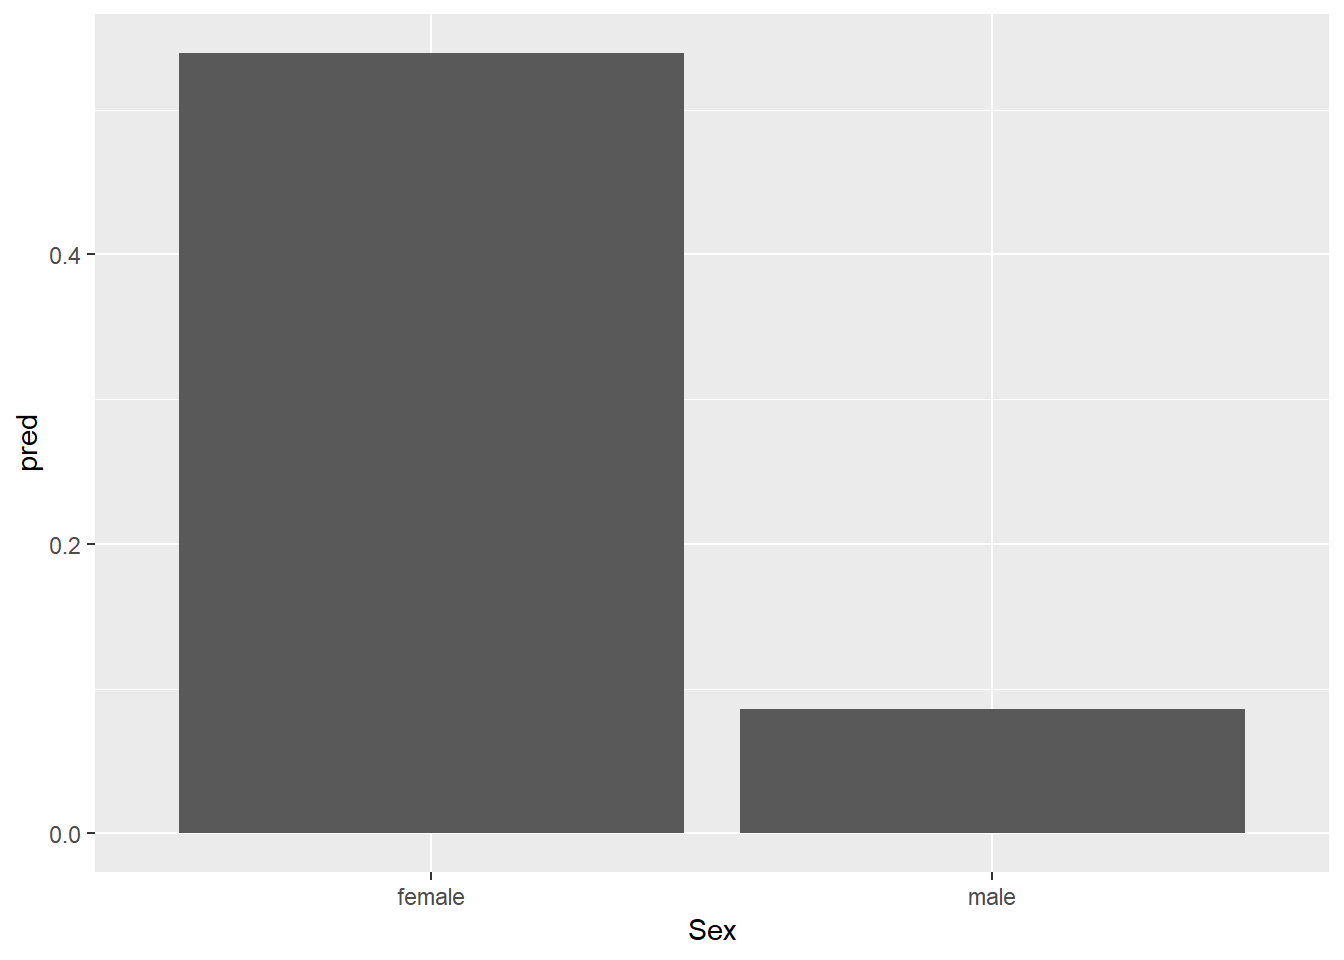
\includegraphics{Bookdown_files/figure-latex/unnamed-chunk-9-1.pdf}

Now let's repeat the process for gender:

\begin{Shaded}
\begin{Highlighting}[]
\NormalTok{pred_gender <-}\StringTok{ }\NormalTok{titanic }\OperatorTok
\StringTok{  }\KeywordTok{data_grid}\NormalTok{(Sex, }\DataTypeTok{.model =}\NormalTok{ model) }\OperatorTok
\StringTok{  }\KeywordTok{filter}\NormalTok{(}\OperatorTok{!}\KeywordTok{is.na}\NormalTok{(Sex))}

\NormalTok{pred_gender }\OperatorTok
\StringTok{  }\KeywordTok{mutate}\NormalTok{(}\DataTypeTok{pred =} \KeywordTok{predict}\NormalTok{(model, }\DataTypeTok{newdata =}\NormalTok{ pred_gender, }\DataTypeTok{type =} \StringTok{"response"}\NormalTok{)) }\OperatorTok
\StringTok{  }\KeywordTok{ggplot}\NormalTok{(}\KeywordTok{aes}\NormalTok{(}\DataTypeTok{x =}\NormalTok{ Sex, }\DataTypeTok{y =}\NormalTok{ pred)) }\OperatorTok{+}
\StringTok{  }\KeywordTok{geom_col}\NormalTok{()}
\end{Highlighting}
\end{Shaded}

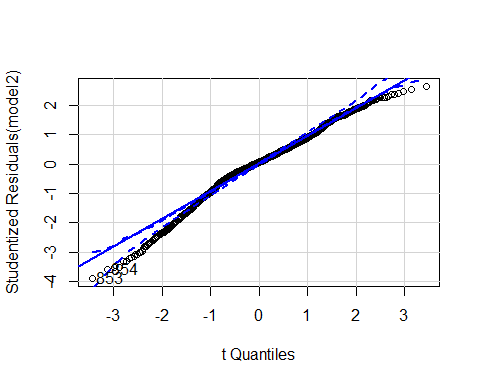
\includegraphics{Bookdown_files/figure-latex/unnamed-chunk-10-1.pdf}

Basically, don't be a guy if you want to survive.

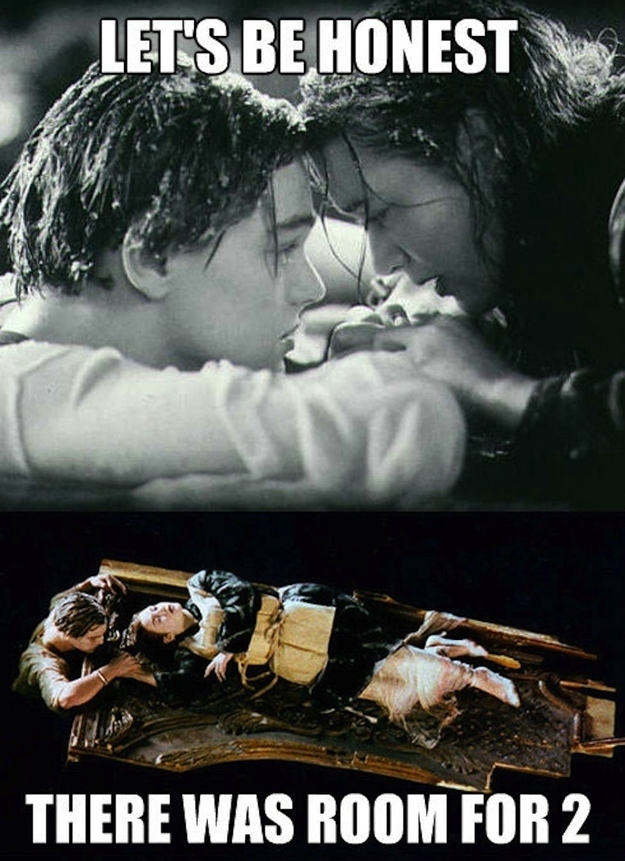
\includegraphics{titanic_meme.jpg} \textless{}\center\textgreater{}

\section{How did our model do?}\label{how-did-our-model-do}

One fun way to see how the model performs is to look at a confusion
matrix. To create a confusion matrix, have hte model spit out
probabilities on the actual data. Then create a new variable that is
equal to 1 if the probability is .50 or higher and 0 otherwise. Then you
simply have a table that compares the predicted outcome (1,0) to the
actual (1,0). The ones that are in the top left and bottom right are the
ones that the model correctly predicted, with the other two spots as the
mis-classifications.

\begin{Shaded}
\begin{Highlighting}[]
\NormalTok{confusion <-}\StringTok{ }\NormalTok{titanic }

\NormalTok{prediction <-}\StringTok{ }\KeywordTok{predict}\NormalTok{(model, confusion, }\DataTypeTok{type =} \StringTok{"response"}\NormalTok{)}

\NormalTok{predicted_classes <-}\StringTok{ }\KeywordTok{ifelse}\NormalTok{(prediction }\OperatorTok{>}\StringTok{ }\FloatTok{0.5}\NormalTok{, }\DecValTok{1}\NormalTok{, }\DecValTok{0}\NormalTok{)}

\NormalTok{predicted_classes <-}\StringTok{ }\KeywordTok{as.factor}\NormalTok{(predicted_classes)}

\KeywordTok{table}\NormalTok{(titanic}\OperatorTok{$}\NormalTok{Survived, predicted_classes)}
\end{Highlighting}
\end{Shaded}

\begin{verbatim}
##    predicted_classes
##       0   1
##   0 356  68
##   1  83 207
\end{verbatim}

In this case our model correct guessed 356 people not surviving and 207
people as surviving. It incorrectly guessed at 83 would die that
actually survived and 68 as surviving who actually died. If we take the
correct over total we get the following:

\begin{Shaded}
\begin{Highlighting}[]
\NormalTok{(}\DecValTok{356} \OperatorTok{+}\StringTok{ }\DecValTok{207}\NormalTok{)}\OperatorTok{/}\NormalTok{(}\DecValTok{356} \OperatorTok{+}\StringTok{ }\DecValTok{207} \OperatorTok{+}\StringTok{ }\DecValTok{83} \OperatorTok{+}\StringTok{ }\DecValTok{68}\NormalTok{)}
\end{Highlighting}
\end{Shaded}

\begin{verbatim}
## [1] 0.7885154
\end{verbatim}

So we can correctly predict 78.8\%. This is a good improvement than if
we just guessed everyone drowned (the model category).

\begin{Shaded}
\begin{Highlighting}[]
\KeywordTok{table}\NormalTok{(titanic}\OperatorTok{$}\NormalTok{Survived)}
\end{Highlighting}
\end{Shaded}

\begin{verbatim}
## 
##   0   1 
## 549 342
\end{verbatim}

\begin{Shaded}
\begin{Highlighting}[]
\DecValTok{549}\OperatorTok{/}\NormalTok{(}\DecValTok{549} \OperatorTok{+}\StringTok{ }\DecValTok{342}\NormalTok{)}
\end{Highlighting}
\end{Shaded}

\begin{verbatim}
## [1] 0.6161616
\end{verbatim}

\section{Final Words}\label{final-words}

This introduction ignored the assumptions that underly logit models. We
also ignored probit models. For a better understanding of how these
models work, I recommend ``Regression Models for Categorical and Limited
Dpeendent Variables'' by J. Scott Long

\section{Data and Packages}\label{data-and-packages}

\begin{Shaded}
\begin{Highlighting}[]
\KeywordTok{library}\NormalTok{(tidyverse)}
\KeywordTok{library}\NormalTok{(modelr)}
\KeywordTok{library}\NormalTok{(haven)}
\KeywordTok{library}\NormalTok{(broom)}

\NormalTok{satisfaction <-}\StringTok{ }\KeywordTok{read_dta}\NormalTok{(}\StringTok{"http://j.mp/SINGHejpr"}\NormalTok{)}
\end{Highlighting}
\end{Shaded}

In this dataset we want to model each respondent's level of satisfaction
with democracy. This variable can be a 1, 2, 3, 4. We can say they are
ordered, but we don't know the distance. 4 is Very satisfied. Because
they are ordered, we should run an ordered logit/probit.

\section{Running the Model}\label{running-the-model}

We will likely want to use the polr (proportional odds logistic
regression) command from the MASS package.

\begin{Shaded}
\begin{Highlighting}[]
\KeywordTok{library}\NormalTok{(MASS)}
\KeywordTok{library}\NormalTok{(effects)}

\NormalTok{satisfaction}\OperatorTok{$}\NormalTok{satisfaction <-}\StringTok{ }\KeywordTok{ordered}\NormalTok{(}\KeywordTok{as.factor}\NormalTok{(satisfaction}\OperatorTok{$}\NormalTok{satisfaction))}

\NormalTok{ideology_satis <-}\StringTok{ }\KeywordTok{polr}\NormalTok{(satisfaction }\OperatorTok{~}\StringTok{ }\NormalTok{voted_ideo}\OperatorTok{*}\NormalTok{winner }\OperatorTok{+}\StringTok{ }\NormalTok{abstained }\OperatorTok{+}
\StringTok{                         }\NormalTok{educ }\OperatorTok{+}\StringTok{ }\NormalTok{efficacy }\OperatorTok{+}\StringTok{ }\NormalTok{majoritarian_prez }\OperatorTok{+}\StringTok{ }\NormalTok{freedom }\OperatorTok{+}\StringTok{ }\NormalTok{gdppercapPPP }\OperatorTok{+}
\StringTok{                         }\NormalTok{gdpgrowth }\OperatorTok{+}\StringTok{ }\NormalTok{CPI }\OperatorTok{+}\StringTok{ }\NormalTok{prez,}
                       \DataTypeTok{method =} \StringTok{"logistic"}\NormalTok{, }\DataTypeTok{data =}\NormalTok{ satisfaction)}
\KeywordTok{summary}\NormalTok{(ideology_satis)}
\end{Highlighting}
\end{Shaded}

\begin{verbatim}
## 
## Re-fitting to get Hessian
\end{verbatim}

\begin{verbatim}
## Call:
## polr(formula = satisfaction ~ voted_ideo * winner + abstained + 
##     educ + efficacy + majoritarian_prez + freedom + gdppercapPPP + 
##     gdpgrowth + CPI + prez, data = satisfaction, method = "logistic")
## 
## Coefficients:
##                      Value Std. Error  t value
## voted_ideo        -0.02170   0.023596  -0.9198
## winner             0.21813   0.020638  10.5694
## abstained         -0.25425   0.020868 -12.1838
## educ               0.08238   0.020180   4.0824
## efficacy           0.16246   0.006211  26.1569
## majoritarian_prez  0.05705   0.018049   3.1609
## freedom            0.04770   0.014087   3.3863
## gdppercapPPP       0.01975   0.001385  14.2578
## gdpgrowth          0.06653   0.003188  20.8673
## CPI               -0.23153   0.005810 -39.8537
## prez              -0.11503   0.026185  -4.3930
## voted_ideo:winner  0.19004   0.037294   5.0957
## 
## Intercepts:
##     Value    Std. Error t value 
## 1|2  -2.0501   0.0584   -35.1284
## 2|3  -0.0588   0.0575    -1.0228
## 3|4   2.7315   0.0586    46.6423
## 
## Residual Deviance: 146397.33 
## AIC: 146427.33
\end{verbatim}

Note that the polr command requires that our outcome variable is ordered
numerically. Also notice the interaction term. While the output shows
t-values, they are actually z values since maximum likelihood methods
typically call for z ratios. Lastly, note the different intercept
cutpoints. These are generally not of interest to us, but are useful
when it comes to making predictions.

If we wanted to get the p-value of a specific variable
(voted\_ideo:winner for instance) then we could run the following code
with the z ratio.

\begin{Shaded}
\begin{Highlighting}[]
\DecValTok{1} \OperatorTok{-}\StringTok{ }\KeywordTok{pnorm}\NormalTok{(}\FloatTok{5.0957}\NormalTok{)}
\end{Highlighting}
\end{Shaded}

\begin{verbatim}
## [1] 1.737275e-07
\end{verbatim}

We can conclude with 99.9\% confidence that the coefficient on the
interaction term is greater than zero.

A nice teature of using the logit link function is that the results can
be inerpreted in terms of odd ratios, though they have to be computed
differently for ordinal models compared to logit models. FOr logit
models, we must exponentiate the negative value of a coefficient and
interpret the odds of being in lower groups relative to higher groups.
For example: the odds ratio for our coefficients from the model above
can be produced by the following code:

\begin{Shaded}
\begin{Highlighting}[]
\DecValTok{100}\OperatorTok{*}\NormalTok{(}\KeywordTok{exp}\NormalTok{(}\OperatorTok{-}\NormalTok{ideology_satis}\OperatorTok{$}\NormalTok{coefficients)}\OperatorTok{-}\DecValTok{1}\NormalTok{)}
\end{Highlighting}
\end{Shaded}

\begin{verbatim}
##        voted_ideo            winner         abstained              educ 
##          2.194186        -19.597657         28.949139         -7.908003 
##          efficacy majoritarian_prez           freedom      gdppercapPPP 
##        -14.994659         -5.545347         -4.658313         -1.955471 
##         gdpgrowth               CPI              prez voted_ideo:winner 
##         -6.436961         26.053177         12.190773        -17.307376
\end{verbatim}

If, for instance, we wanted to interpret the influence of efficiency,
then we could say that for a one point incrase on a five point efficacy
scale, the odds a respondent will report that they are ``not at all
satisfied'' with democracy relative to any of the three categories
decrease by 15\%, all else equal. Also, the odds that a respondent will
report ``not at all satisfied'' or ``not very satisfied'' relative to
the two higher categories also decrease by 15\%, all else equal. In
general then, we can interpret the oddds ratio for an ordered logit as
shaping the odds of all optiosn below a threshold relative to all
options above a threshold.

\section{Gettin predictions:}\label{gettin-predictions}

Here I am doing the discrete class predicted, not the predicted
probabilities. If you want to see predicted probabilities, see the
section of \texttt{Graphing\ the\ Tidy\ Way}.

Somewhat uninteresting is that all of them are expected to be in the 3rd
category.

\begin{Shaded}
\begin{Highlighting}[]
\NormalTok{new_data <-}\StringTok{ }\NormalTok{satisfaction }\OperatorTok
\StringTok{  }\KeywordTok{data_grid}\NormalTok{(efficacy, }\DataTypeTok{.model =}\NormalTok{ ideology_satis)}
  

\NormalTok{new_data <-}\StringTok{ }\NormalTok{new_data }\OperatorTok
\StringTok{  }\KeywordTok{mutate}\NormalTok{(}\DataTypeTok{pred_class =} \KeywordTok{predict}\NormalTok{(ideology_satis, new_data, }\DataTypeTok{type =} \StringTok{"class"}\NormalTok{))}

\NormalTok{new_data}
\end{Highlighting}
\end{Shaded}

\begin{verbatim}
## # A tibble: 5 x 12
##   efficacy voted_ideo winner abstained  educ majoritarian_pr~ freedom
##      <dbl>      <dbl>  <dbl>     <dbl> <dbl>            <dbl>   <dbl>
## 1        1          0      0         0     0                0      -1
## 2        2          0      0         0     0                0      -1
## 3        3          0      0         0     0                0      -1
## 4        4          0      0         0     0                0      -1
## 5        5          0      0         0     0                0      -1
## # ... with 5 more variables: gdppercapPPP <dbl>, gdpgrowth <dbl>,
## #   CPI <dbl>, prez <dbl>, pred_class <fct>
\end{verbatim}

\chapter{Showing predictions}\label{showing-predictions}

\begin{Shaded}
\begin{Highlighting}[]
\KeywordTok{Effect}\NormalTok{(}\DataTypeTok{focal.predictors =} \KeywordTok{c}\NormalTok{(}\StringTok{"voted_ideo"}\NormalTok{, }\StringTok{"winner"}\NormalTok{), ideology_satis)}
\end{Highlighting}
\end{Shaded}

\begin{verbatim}
## 
## Re-fitting to get Hessian
\end{verbatim}

\begin{verbatim}
## 
## voted_ideo*winner effect (probability) for 1
##           winner
## voted_ideo          0        0.2        0.5        0.8          1
##        0   0.07738718 0.07432926 0.06995037 0.06581111 0.06317929
##        0.2 0.07769769 0.07410523 0.06900243 0.06422663 0.06121568
##        0.5 0.07816558 0.07377033 0.06760280 0.06191642 0.05837700
##        0.8 0.07863605 0.07343684 0.06622953 0.05968401 0.05566216
##        1   0.07895114 0.07321528 0.06532847 0.05823785 0.05391873
## 
## voted_ideo*winner effect (probability) for 2
##           winner
## voted_ideo         0       0.2       0.5       0.8         1
##        0   0.3031896 0.2960183 0.2852714 0.2745687 0.2674749
##        0.2 0.3039029 0.2954823 0.2828681 0.2703255 0.2620302
##        0.5 0.3049728 0.2946783 0.2792682 0.2639884 0.2539215
##        0.8 0.3060424 0.2938744 0.2756754 0.2576905 0.2458946
##        1   0.3067553 0.2933386 0.2732849 0.2535167 0.2405948
## 
## voted_ideo*winner effect (probability) for 3
##           winner
## voted_ideo         0       0.2       0.5       0.8         1
##        0   0.5285674 0.5351282 0.5445027 0.5532844 0.5587926
##        0.2 0.5279015 0.5356088 0.5465232 0.5566096 0.5628467
##        0.5 0.5268982 0.5363271 0.5494974 0.5614062 0.5685967
##        0.8 0.5258898 0.5370422 0.5524023 0.5659676 0.5739373
##        1   0.5252147 0.5375173 0.5542999 0.5688746 0.5772640
## 
## voted_ideo*winner effect (probability) for 4
##           winner
## voted_ideo          0        0.2       0.5       0.8         1
##        0   0.09085585 0.09452425 0.1002756 0.1063358 0.1105532
##        0.2 0.09049792 0.09480369 0.1016063 0.1088383 0.1139074
##        0.5 0.08996341 0.09522425 0.1036317 0.1126889 0.1191048
##        0.8 0.08943174 0.09564648 0.1056927 0.1166580 0.1245060
##        1   0.08907887 0.09592889 0.1070867 0.1193709 0.1282225
\end{verbatim}

\begin{Shaded}
\begin{Highlighting}[]
\KeywordTok{plot}\NormalTok{(}\KeywordTok{Effect}\NormalTok{(}\DataTypeTok{focal.predictors =} \KeywordTok{c}\NormalTok{(}\StringTok{"voted_ideo"}\NormalTok{, }\StringTok{"winner"}\NormalTok{), ideology_satis))}
\end{Highlighting}
\end{Shaded}

\begin{verbatim}
## 
## Re-fitting to get Hessian
\end{verbatim}

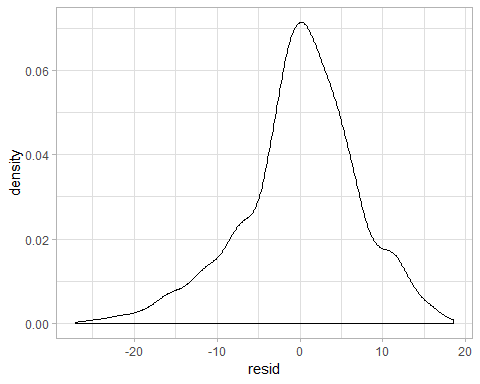
\includegraphics{Bookdown_files/figure-latex/unnamed-chunk-20-1.pdf}

\begin{Shaded}
\begin{Highlighting}[]
\KeywordTok{plot}\NormalTok{(}\KeywordTok{Effect}\NormalTok{(}\DataTypeTok{focal.predictors =} \StringTok{"efficacy"}\NormalTok{, ideology_satis))}
\end{Highlighting}
\end{Shaded}

\begin{verbatim}
## 
## Re-fitting to get Hessian
\end{verbatim}

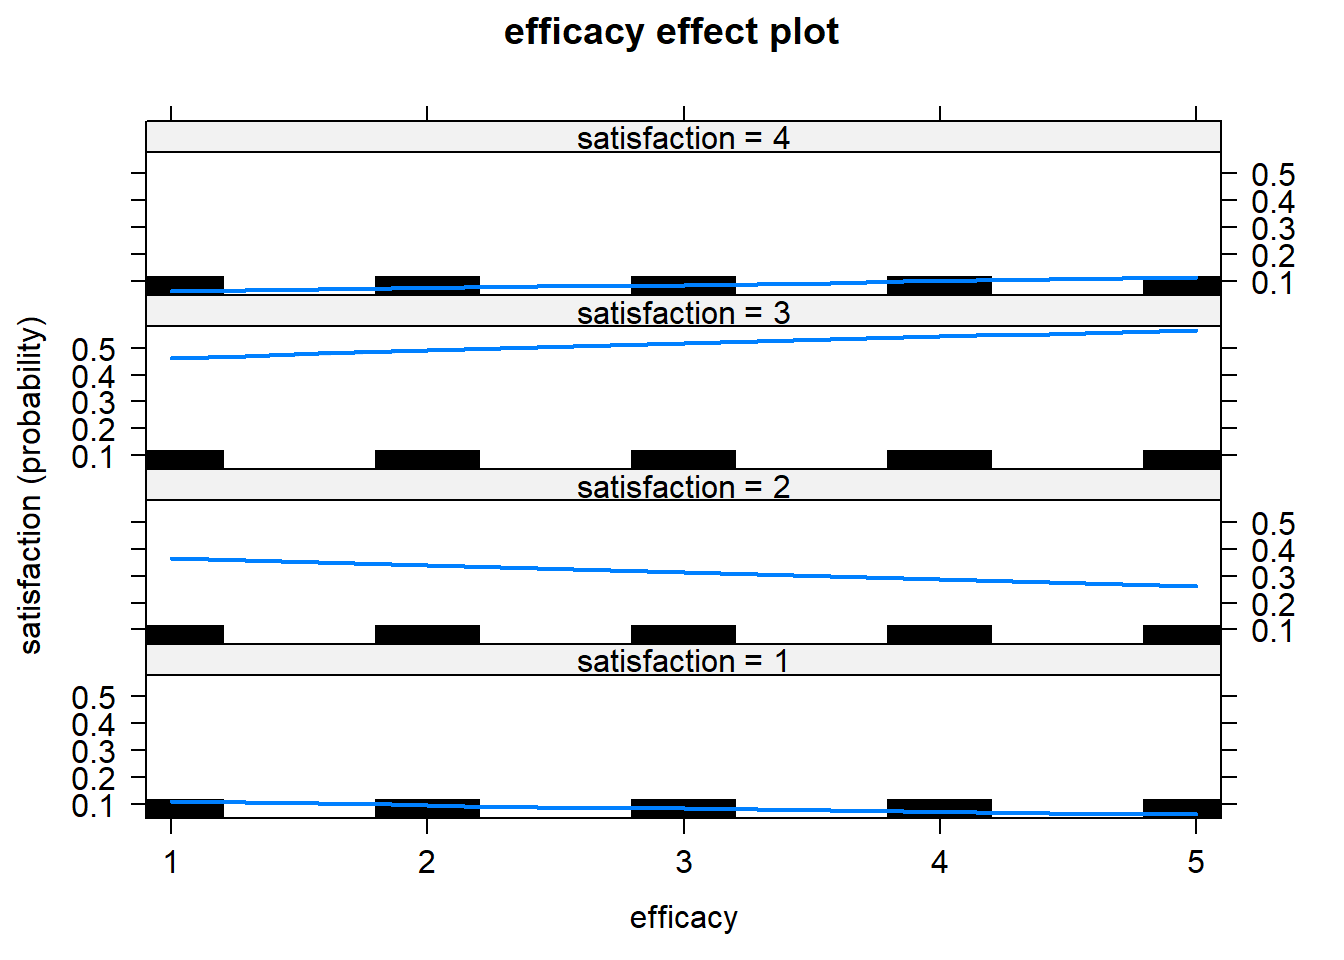
\includegraphics{Bookdown_files/figure-latex/unnamed-chunk-21-1.pdf}

\chapter{Graphing in a Tidy Way}\label{graphing-in-a-tidy-way}

I am not sure if I have greally graphed this correctly, but this is what
I could come up with.

\begin{Shaded}
\begin{Highlighting}[]
\NormalTok{pred <-}\StringTok{ }\KeywordTok{predict}\NormalTok{(ideology_satis, }\DataTypeTok{type =} \StringTok{"probs"}\NormalTok{)}


\NormalTok{prediction <-}\StringTok{ }\KeywordTok{cbind}\NormalTok{(satisfaction, pred)}


\NormalTok{prediction }\OperatorTok
\StringTok{  }\KeywordTok{rename}\NormalTok{(}\StringTok{"one"}\NormalTok{ =}\StringTok{ }\DecValTok{22}\NormalTok{,}
         \StringTok{"two"}\NormalTok{ =}\StringTok{ }\DecValTok{23}\NormalTok{,}
         \StringTok{"three"}\NormalTok{ =}\StringTok{ }\DecValTok{24}\NormalTok{,}
         \StringTok{"four"}\NormalTok{ =}\StringTok{ }\DecValTok{25}\NormalTok{) }\OperatorTok
\StringTok{  }\NormalTok{dplyr}\OperatorTok{::}\KeywordTok{select}\NormalTok{(efficacy, one, two, three, four) }\OperatorTok
\StringTok{  }\KeywordTok{gather}\NormalTok{(outcome, prediction, }\OperatorTok{-}\NormalTok{efficacy) }\OperatorTok
\StringTok{  }\KeywordTok{mutate}\NormalTok{(}\DataTypeTok{outcome =} \KeywordTok{factor}\NormalTok{(outcome, }\DataTypeTok{levels =} \KeywordTok{c}\NormalTok{(}\StringTok{"one"}\NormalTok{, }\StringTok{"two"}\NormalTok{, }\StringTok{"three"}\NormalTok{, }\StringTok{"four"}\NormalTok{))) }\OperatorTok
\StringTok{  }\KeywordTok{ggplot}\NormalTok{(}\KeywordTok{aes}\NormalTok{(}\DataTypeTok{x =}\NormalTok{ prediction, }\DataTypeTok{fill =} \KeywordTok{as.factor}\NormalTok{(efficacy))) }\OperatorTok{+}
\StringTok{  }\KeywordTok{geom_histogram}\NormalTok{() }\OperatorTok{+}
\StringTok{  }\KeywordTok{facet_wrap}\NormalTok{(efficacy}\OperatorTok{~}\NormalTok{outcome, }\DataTypeTok{ncol =} \DecValTok{4}\NormalTok{) }\OperatorTok{+}
\StringTok{  }\KeywordTok{labs}\NormalTok{(}\DataTypeTok{fill =} \StringTok{"Efficacy Levels"}\NormalTok{)}
\end{Highlighting}
\end{Shaded}

\begin{verbatim}
## `stat_bin()` using `bins = 30`. Pick better value with `binwidth`.
\end{verbatim}

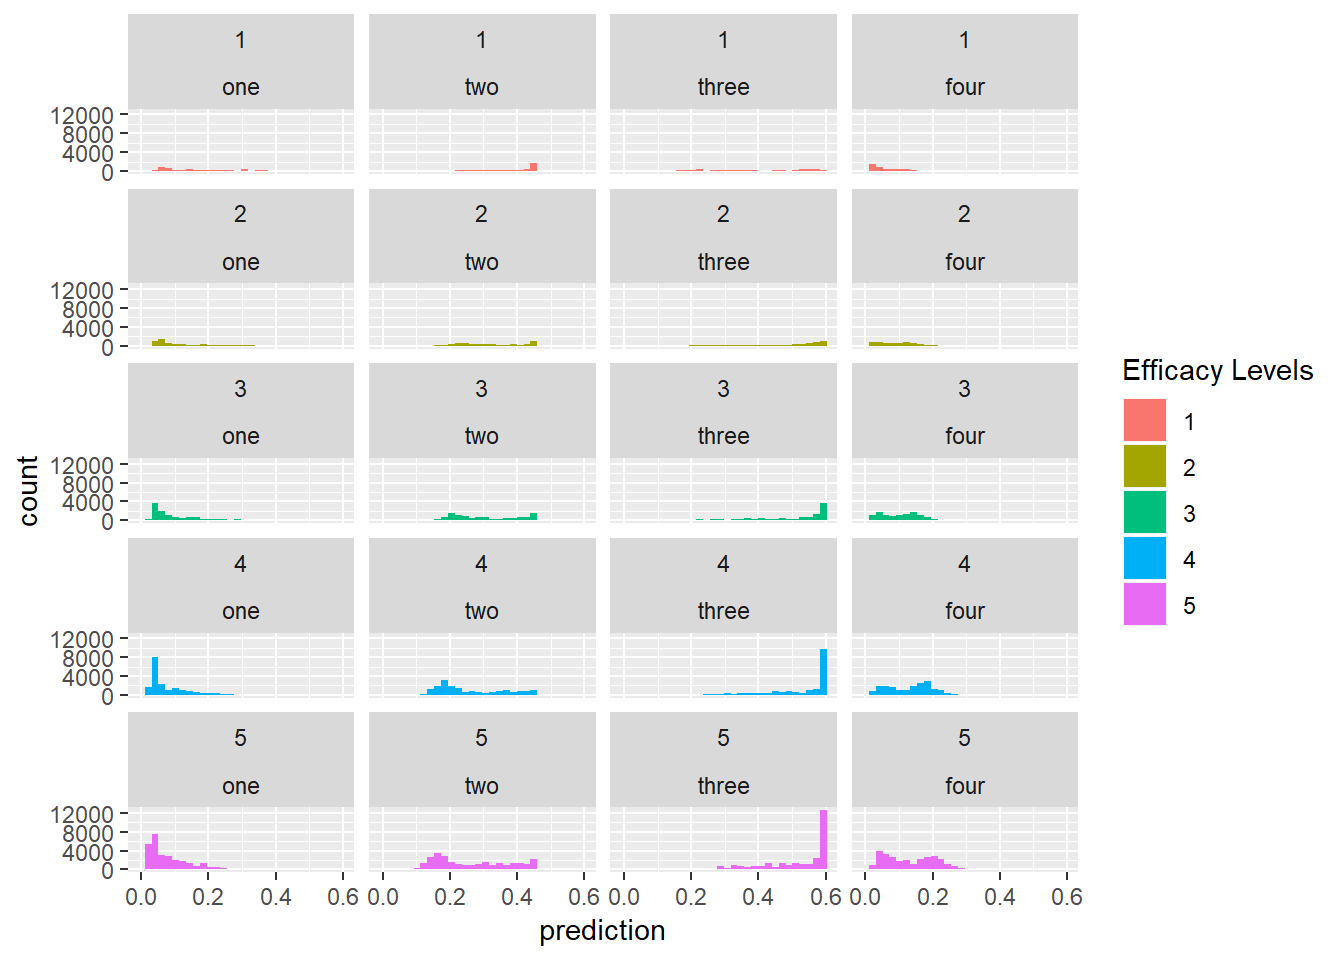
\includegraphics{Bookdown_files/figure-latex/unnamed-chunk-22-1.pdf}

\section{DataCamp tutorial}\label{datacamp-tutorial}

\begin{Shaded}
\begin{Highlighting}[]
\KeywordTok{library}\NormalTok{(lme4)}
\KeywordTok{library}\NormalTok{(foreign)}
\KeywordTok{library}\NormalTok{(broom)}
\KeywordTok{library}\NormalTok{(tidyverse)}
\end{Highlighting}
\end{Shaded}

\emph{Fixed-effect} parameters only use data for a specific group. In
contrast, \emph{random-effect} parameters assume data share a common
distribution. FOr situations with small amounts of data or ourliers,
random effect models can produce different estimates.

\begin{Shaded}
\begin{Highlighting}[]
\NormalTok{evolution<-}\KeywordTok{read.dta}\NormalTok{(}\StringTok{"http://j.mp/BPchap7"}\NormalTok{)}
\NormalTok{evolution}\OperatorTok{$}\NormalTok{female[evolution}\OperatorTok{$}\NormalTok{female}\OperatorTok{==}\DecValTok{9}\NormalTok{]<-}\OtherTok{NA}
\NormalTok{evolution<-}\KeywordTok{subset}\NormalTok{(evolution,}\OperatorTok{!}\KeywordTok{is.na}\NormalTok{(female))}
\end{Highlighting}
\end{Shaded}

\subsection{full model}\label{full-model}

\begin{Shaded}
\begin{Highlighting}[]
\NormalTok{hours_ml<-}\KeywordTok{lmer}\NormalTok{(hrs_allev }\OperatorTok{~}\StringTok{ }\NormalTok{phase1 }\OperatorTok{+}\StringTok{ }\NormalTok{senior_c }\OperatorTok{+}\StringTok{ }\NormalTok{ph_senior }\OperatorTok{+}\StringTok{ }\NormalTok{notest_p }\OperatorTok{+}\StringTok{ }\NormalTok{ph_notest_p }\OperatorTok{+}\StringTok{ }\NormalTok{female }\OperatorTok{+}\StringTok{ }\NormalTok{biocred3 }\OperatorTok{+}\StringTok{ }
\StringTok{                 }\NormalTok{degr3 }\OperatorTok{+}\StringTok{ }\NormalTok{evol_course }\OperatorTok{+}\StringTok{ }\NormalTok{certified }\OperatorTok{+}\StringTok{ }\NormalTok{idsci_trans }\OperatorTok{+}\StringTok{ }\NormalTok{confident }\OperatorTok{+}\StringTok{ }\NormalTok{(}\DecValTok{1}\OperatorTok{|}\NormalTok{st_fip), }\DataTypeTok{data =}\NormalTok{ evolution)}
\end{Highlighting}
\end{Shaded}

\subsection{building the model}\label{building-the-model}

Here we are building a random effects with no fixed effects:

\begin{Shaded}
\begin{Highlighting}[]
\NormalTok{initial <-}\StringTok{ }\KeywordTok{lmer}\NormalTok{(hrs_allev }\OperatorTok{~}\StringTok{ }\NormalTok{(}\DecValTok{1} \OperatorTok{|}\StringTok{ }\NormalTok{st_fip), }\DataTypeTok{data =}\NormalTok{ evolution)}

\KeywordTok{summary}\NormalTok{(initial)}
\end{Highlighting}
\end{Shaded}

\begin{verbatim}
## Linear mixed model fit by REML ['lmerMod']
## Formula: hrs_allev ~ (1 | st_fip)
##    Data: evolution
## 
## REML criterion at convergence: 6049
## 
## Scaled residuals: 
##     Min      1Q  Median      3Q     Max 
## -1.6954 -0.7003 -0.2460  0.6036  3.5975 
## 
## Random effects:
##  Groups   Name        Variance Std.Dev.
##  st_fip   (Intercept)  5.046   2.246   
##  Residual             74.952   8.657   
## Number of obs: 841, groups:  st_fip, 49
## 
## Fixed effects:
##             Estimate Std. Error t value
## (Intercept)   14.222      0.477   29.82
\end{verbatim}

\begin{Shaded}
\begin{Highlighting}[]
\KeywordTok{plot}\NormalTok{(initial)}
\end{Highlighting}
\end{Shaded}

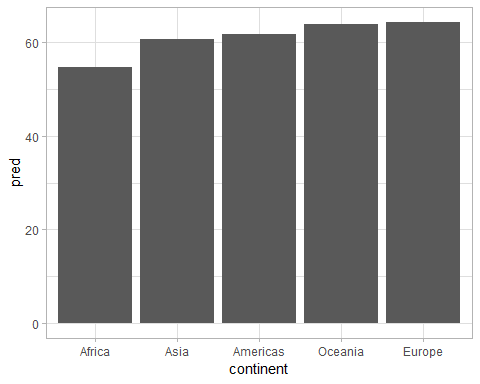
\includegraphics{Bookdown_files/figure-latex/unnamed-chunk-28-1.pdf}

Now let's build one with a fixed-effect slope parameter:

\begin{Shaded}
\begin{Highlighting}[]
\NormalTok{fixed <-}\StringTok{ }\KeywordTok{lmer}\NormalTok{(hrs_allev }\OperatorTok{~}\StringTok{ }\NormalTok{phase1 }\OperatorTok{+}\StringTok{ }\NormalTok{(}\DecValTok{1} \OperatorTok{|}\StringTok{ }\NormalTok{st_fip), }\DataTypeTok{data =}\NormalTok{ evolution)}

\KeywordTok{summary}\NormalTok{(fixed)}
\end{Highlighting}
\end{Shaded}

\begin{verbatim}
## Linear mixed model fit by REML ['lmerMod']
## Formula: hrs_allev ~ phase1 + (1 | st_fip)
##    Data: evolution
## 
## REML criterion at convergence: 6044.3
## 
## Scaled residuals: 
##     Min      1Q  Median      3Q     Max 
## -1.7107 -0.6892 -0.2430  0.6116  3.6573 
## 
## Random effects:
##  Groups   Name        Variance Std.Dev.
##  st_fip   (Intercept)  4.65    2.156   
##  Residual             74.79    8.648   
## Number of obs: 841, groups:  st_fip, 49
## 
## Fixed effects:
##             Estimate Std. Error t value
## (Intercept)  14.2695     0.4672  30.541
## phase1        0.9433     0.4425   2.132
## 
## Correlation of Fixed Effects:
##        (Intr)
## phase1 0.058
\end{verbatim}

Now to add a random slope:

\begin{Shaded}
\begin{Highlighting}[]
\NormalTok{random_slopes <-}\StringTok{ }\KeywordTok{lmer}\NormalTok{(hrs_allev }\OperatorTok{~}\StringTok{ }\NormalTok{phase1 }\OperatorTok{+}\StringTok{ }\NormalTok{(notest_p }\OperatorTok{|}\StringTok{ }\NormalTok{st_fip), }\DataTypeTok{data =}\NormalTok{ evolution)}

\NormalTok{broom}\OperatorTok{::}\KeywordTok{tidy}\NormalTok{(random_slopes)}
\end{Highlighting}
\end{Shaded}

\begin{verbatim}
## # A tibble: 6 x 5
##   term                            estimate std.error statistic group   
##   <chr>                              <dbl>     <dbl>     <dbl> <chr>   
## 1 (Intercept)                       14.3       0.458     31.2  fixed   
## 2 phase1                             0.829     0.424      1.96 fixed   
## 3 sd_(Intercept).st_fip              2.34     NA         NA    st_fip  
## 4 sd_notest_p.st_fip                 0.924    NA         NA    st_fip  
## 5 cor_(Intercept).notest_p.st_fip   -1.000    NA         NA    st_fip  
## 6 sd_Observation.Residual            8.65     NA         NA    Residual
\end{verbatim}

If we wanted to assume uncorrelated random-effect slopes (it is actually
easier to calculate) all we have to do is turn \texttt{\textbar{}} into
\texttt{\textbar{}\textbar{}} (though you likely want a reason to do
this, I am just doing here for instruction)

\begin{Shaded}
\begin{Highlighting}[]
\NormalTok{uncor <-}\StringTok{ }\KeywordTok{lmer}\NormalTok{(hrs_allev }\OperatorTok{~}\StringTok{ }\NormalTok{phase1 }\OperatorTok{+}\StringTok{ }\NormalTok{(notest_p }\OperatorTok{||}\StringTok{ }\NormalTok{st_fip), }\DataTypeTok{data =}\NormalTok{ evolution)}
\end{Highlighting}
\end{Shaded}

\begin{verbatim}
## singular fit
\end{verbatim}

\begin{Shaded}
\begin{Highlighting}[]
\KeywordTok{summary}\NormalTok{(uncor)}
\end{Highlighting}
\end{Shaded}

\begin{verbatim}
## Linear mixed model fit by REML ['lmerMod']
## Formula: hrs_allev ~ phase1 + ((1 | st_fip) + (0 + notest_p | st_fip))
##    Data: evolution
## 
## REML criterion at convergence: 6044.3
## 
## Scaled residuals: 
##     Min      1Q  Median      3Q     Max 
## -1.7107 -0.6892 -0.2430  0.6116  3.6573 
## 
## Random effects:
##  Groups   Name        Variance Std.Dev.
##  st_fip   (Intercept)  4.65    2.156   
##  st_fip.1 notest_p     0.00    0.000   
##  Residual             74.79    8.648   
## Number of obs: 841, groups:  st_fip, 49
## 
## Fixed effects:
##             Estimate Std. Error t value
## (Intercept)  14.2695     0.4672  30.541
## phase1        0.9433     0.4425   2.132
## 
## Correlation of Fixed Effects:
##        (Intr)
## phase1 0.058 
## convergence code: 0
## singular fit
\end{verbatim}

You can also have a variable as a fixed effect while correcting for
random slopes:

\begin{Shaded}
\begin{Highlighting}[]
\NormalTok{fixed_random <-}\StringTok{ }\KeywordTok{lmer}\NormalTok{(hrs_allev }\OperatorTok{~}\StringTok{ }\NormalTok{phase1 }\OperatorTok{+}\StringTok{ }\NormalTok{(phase1 }\OperatorTok{||}\StringTok{ }\NormalTok{st_fip), }\DataTypeTok{data =}\NormalTok{ evolution)}
\end{Highlighting}
\end{Shaded}

\begin{verbatim}
## singular fit
\end{verbatim}

\begin{Shaded}
\begin{Highlighting}[]
\KeywordTok{summary}\NormalTok{(fixed_random)}
\end{Highlighting}
\end{Shaded}

\begin{verbatim}
## Linear mixed model fit by REML ['lmerMod']
## Formula: hrs_allev ~ phase1 + ((1 | st_fip) + (0 + phase1 | st_fip))
##    Data: evolution
## 
## REML criterion at convergence: 6044.3
## 
## Scaled residuals: 
##     Min      1Q  Median      3Q     Max 
## -1.7107 -0.6892 -0.2430  0.6116  3.6573 
## 
## Random effects:
##  Groups   Name        Variance  Std.Dev. 
##  st_fip   (Intercept) 4.650e+00 2.156e+00
##  st_fip.1 phase1      8.776e-09 9.368e-05
##  Residual             7.479e+01 8.648e+00
## Number of obs: 841, groups:  st_fip, 49
## 
## Fixed effects:
##             Estimate Std. Error t value
## (Intercept)  14.2695     0.4672  30.541
## phase1        0.9433     0.4425   2.132
## 
## Correlation of Fixed Effects:
##        (Intr)
## phase1 0.058 
## convergence code: 0
## singular fit
\end{verbatim}

\chapter{Understanding and reporting the
outputs}\label{understanding-and-reporting-the-outputs}

Point estimates

\begin{Shaded}
\begin{Highlighting}[]
\KeywordTok{fixef}\NormalTok{(fixed_random)}
\end{Highlighting}
\end{Shaded}

\begin{verbatim}
## (Intercept)      phase1 
##  14.2695219   0.9433342
\end{verbatim}

\begin{Shaded}
\begin{Highlighting}[]
\KeywordTok{ranef}\NormalTok{(fixed_random)}
\end{Highlighting}
\end{Shaded}

\begin{verbatim}
## $st_fip
##    (Intercept)        phase1
## 1  -1.78282438  4.597615e-09
## 2   1.15330874  4.377183e-10
## 4   0.12852444  1.930166e-10
## 5  -2.35878914 -1.237115e-09
## 6   0.23091628  4.199415e-10
## 8   2.66045865 -3.606000e-10
## 9  -1.33099385 -2.003182e-09
## 10  0.49232783  2.746547e-10
## 12  0.10160073 -4.770269e-10
## 13  0.05943937  4.113800e-12
## 15 -0.17678200 -2.654893e-10
## 16  0.28163119  1.562015e-10
## 17  2.17846498 -1.022814e-08
## 18  1.65088717  2.479285e-09
## 19 -0.69394682  3.258159e-09
## 20 -0.63451950 -5.529394e-10
## 21  1.87521347 -1.524100e-09
## 22 -1.50389226  1.641151e-10
## 23  1.78044856 -5.773276e-09
## 24  0.17909278  6.855145e-11
## 25  1.39501625  1.648564e-09
## 26 -1.78177645 -4.237651e-10
## 27 -0.08529162  9.307610e-12
## 28 -1.97456015  6.096326e-09
## 29 -0.94328552 -1.712393e-09
## 30  0.20095069 -8.624070e-11
## 31 -0.13355239 -7.450480e-11
## 32  2.70958201  4.069221e-09
## 33  1.27133656  1.913396e-09
## 34 -0.89252671 -2.122723e-10
## 35 -0.35287129 -5.310809e-10
## 36 -0.59671918 -1.646509e-09
## 37 -2.18153661 -3.269144e-09
## 38  1.09443772  2.602933e-10
## 39  0.72371535  1.316140e-09
## 40  0.37463919 -1.758973e-09
## 41  1.67672441  1.167555e-09
## 42 -1.01339149 -5.282123e-10
## 44  0.84611504  5.891763e-10
## 45  2.29931998  2.003697e-09
## 46  0.07315518 -1.309536e-10
## 47 -3.15737613 -2.198579e-09
## 48 -2.67912474  3.017555e-09
## 49 -0.57052531 -1.216445e-09
## 50 -0.39149904 -3.280883e-10
## 51 -0.60100189  1.559923e-09
## 53  0.41503195 -4.663502e-11
## 54 -1.20583697  5.980493e-10
## 55  1.19028491  2.830890e-10
## 
## with conditional variances for "st_fip"
\end{verbatim}

We can also get confidence interals for the fixed effects using
confint()

\begin{Shaded}
\begin{Highlighting}[]
\KeywordTok{confint}\NormalTok{(fixed_random)}
\end{Highlighting}
\end{Shaded}

\begin{verbatim}
## Computing profile confidence intervals ...
\end{verbatim}

\begin{verbatim}
##                  2.5 %    97.5 %
## .sig01       1.0590439  3.162650
## .sig02       0.0000000  1.802257
## .sigma       8.2414661  9.095810
## (Intercept) 13.3612218 15.205404
## phase1       0.0835454  1.893044
\end{verbatim}

Using the broom.mixed package, you can use the \texttt{tidy()} function
to extract model results, though this isn't as tidy as most models are:

\begin{Shaded}
\begin{Highlighting}[]
\KeywordTok{library}\NormalTok{(broom)}

\KeywordTok{tidy}\NormalTok{(fixed_random, }\DataTypeTok{conf.int =} \OtherTok{TRUE}\NormalTok{)}
\end{Highlighting}
\end{Shaded}

\begin{verbatim}
## # A tibble: 5 x 7
##   term               estimate std.error statistic conf.low conf.high group 
##   <chr>                 <dbl>     <dbl>     <dbl>    <dbl>     <dbl> <chr> 
## 1 (Intercept)      14.3           0.467     30.5   13.4        15.2  fixed 
## 2 phase1            0.943         0.442      2.13   0.0761      1.81 fixed 
## 3 sd_(Intercept).~  2.16         NA         NA     NA          NA    st_fip
## 4 sd_phase1.st_fi~  0.0000937    NA         NA     NA          NA    st_fi~
## 5 sd_Observation.~  8.65         NA         NA     NA          NA    Resid~
\end{verbatim}

\section{Communicating results}\label{communicating-results}

This is not very easy to extract lmer results (see
\href{https://github.com/tidymodels/broom/issues/96}{link}).

\begin{Shaded}
\begin{Highlighting}[]
\CommentTok{# Extract out the parameter estimates and confidence intervals and manipulate the data}
\NormalTok{dataPlot <-}\StringTok{ }\KeywordTok{data.frame}\NormalTok{(}\KeywordTok{cbind}\NormalTok{( }\KeywordTok{fixef}\NormalTok{(fixed_random), }\KeywordTok{confint}\NormalTok{(fixed_random)[ }\DecValTok{4}\OperatorTok{:}\DecValTok{5}\NormalTok{, ])) }\CommentTok{# getting the rows for confint}
\end{Highlighting}
\end{Shaded}

\begin{verbatim}
## Computing profile confidence intervals ...
\end{verbatim}

\begin{Shaded}
\begin{Highlighting}[]
\KeywordTok{rownames}\NormalTok{(dataPlot)[}\DecValTok{1}\NormalTok{] <-}\StringTok{ "Intercept"}
\KeywordTok{colnames}\NormalTok{(dataPlot) <-}\StringTok{ }\KeywordTok{c}\NormalTok{(}\StringTok{"est"}\NormalTok{, }\StringTok{"L95"}\NormalTok{, }\StringTok{"U95"}\NormalTok{)}
\NormalTok{dataPlot}\OperatorTok{$}\NormalTok{parameter <-}\StringTok{ }\KeywordTok{rownames}\NormalTok{(dataPlot)}

\CommentTok{# Print the new dataframe}
\KeywordTok{print}\NormalTok{(dataPlot)}
\end{Highlighting}
\end{Shaded}

\begin{verbatim}
##                  est        L95       U95 parameter
## Intercept 14.2695219 13.3612218 15.205404 Intercept
## phase1     0.9433342  0.0835454  1.893044    phase1
\end{verbatim}

\begin{Shaded}
\begin{Highlighting}[]
\CommentTok{# Plot the results using ggplot2}
\KeywordTok{ggplot}\NormalTok{(dataPlot, }\KeywordTok{aes}\NormalTok{(}\DataTypeTok{x =}\NormalTok{ parameter, }\DataTypeTok{y =}\NormalTok{ est, }\DataTypeTok{ymin =}\NormalTok{ L95, }\DataTypeTok{ymax =}\NormalTok{ U95)) }\OperatorTok{+}
\StringTok{  }\KeywordTok{geom_hline}\NormalTok{( }\DataTypeTok{yintercept =} \DecValTok{0}\NormalTok{, }\DataTypeTok{color =} \StringTok{'red'}\NormalTok{ ) }\OperatorTok{+}
\StringTok{  }\KeywordTok{geom_linerange}\NormalTok{() }\OperatorTok{+}\StringTok{ }
\StringTok{  }\KeywordTok{geom_point}\NormalTok{() }\OperatorTok{+}\StringTok{ }
\StringTok{  }\KeywordTok{coord_flip}\NormalTok{() }\OperatorTok{+}\StringTok{ }
\StringTok{  }\KeywordTok{theme_minimal}\NormalTok{()}
\end{Highlighting}
\end{Shaded}

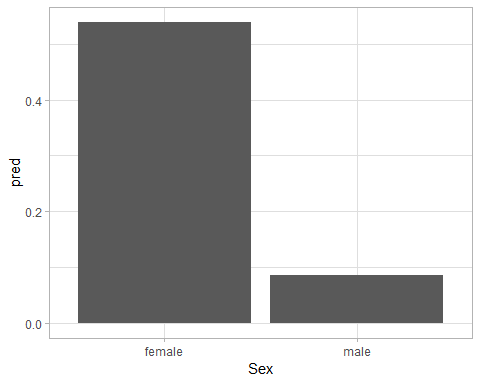
\includegraphics{Bookdown_files/figure-latex/unnamed-chunk-37-1.pdf}

\chapter{Statistical Inference with Maryland Crime
Data}\label{statistical-inference-with-maryland-crime-data}

\bibliography{book.bib,packages.bib}


\end{document}
